% To be included at the beginning

\documentclass[,dvipsnames,a4paper, oneside]{ctexart}
\pagestyle{plain}               %去掉header
% CTEXart 默认section 居中, 用如下redefine, 但我们直接renewcommand
% \CTEXsetup[format={\Large\bfseries}]{section}

\title{周报}
\usepackage{geometry}
\newgeometry{
  total={170mm,257mm},
  left=20mm,
  top=20mm,
}
\author{丛坚而}
\date{\today}

% 注意一点:含有 @ 的命令是内部命令,不需要立即执行,需
% 要配合 \makeatletter ... \makeatother延迟,之后再执行。

\newcommand{\mycol}{gray}
\newcommand{\mycoli}{NavyBlue}
\usepackage{tikz}

\makeatletter % change default title style
% \newtcbox{\datebox}[1][\mycoli]{
% }
\renewcommand*\maketitle{%
  {
    % \noindent \LARGE
    \tcbox[
    nobeforeafter,
    top=2cm,tile,colback=gray!50!black,coltext=white,spread upwards
    ]
    {\Large \bfseries \@title}
    \hfill
    % \datebox{\bfseries % 默认粗体
    %   \large \@date}
    \tcbox[on line,
    arc=0pt, outer arc=0pt, colback=\mycol!10!white,colframe=\mycoli!50!black,
    boxsep=0pt,left=1pt,right=1pt,top=2pt,bottom=2pt,
    boxrule=0pt,bottomrule=1pt,toprule=1pt]{\@date}
   \par
    } % LARGE字号
    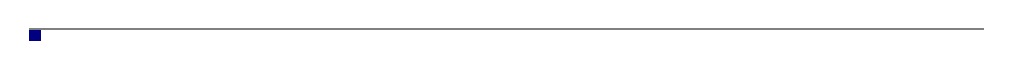
\begin{tikzpicture}
      \fill[\mycoli] (1ex,0) rectangle +(-1ex,-1ex);
      \draw[thick,draw=\mycol] (0,0) -- (\textwidth,0);
    \end{tikzpicture}
    \vskip 1em% %%%  标题下面只有1em的缩进或margin
}
\makeatother

\makeatletter % change default title style
\newcommand\makeend{%
  \vskip 2em
  
\begin{tikzpicture}
    % \fill[\mycol] (\textwidth,0ex) rectangle +(-1ex,-1ex);
    \fill[\mycol] (0ex,0ex) rectangle +(1ex,-1ex); %square on the left
    \draw[thick,draw=\mycoli] (0,0) -- (\textwidth,0);
  \end{tikzpicture}

  % \RaggedLeftLeftskip=0pt plus 1fil %the left fill for FlushRight
  % \RaggedLeftRightskip=5em          %the right skip for FlushRight
  % \begin{FlushRight}
  %   % 本周报告完毕\\
  %   % 报告人:\@author%
  % \end{FlushRight}

  \vskip 1em
  \begin{tcolorbox}[enhanced,nobeforeafter,
  right=2cm,tile,colback=\mycoli!20!black,coltext=white,
  % capture=minipage,
  spread inwards,
  grow to left by=-13cm
  ]
  {
    \bfseries
    本周报告完毕\\
    报告人:\@author%
  }
\end{tcolorbox}
}

% Use titlesec pkg instead 

%% Box the \section
% \renewcommand{\section}{%
%   \@startsection%
%   {section}
%   {1}{0pt}
%   {5ex}{1ex plus .2ex}
%   {\large%
%     \def\h{1ex}
%     \def\w{1ex}
%     \tikz\fill[NavyBlue] (0,-\h)--(\w,0)--(0,\h)--cycle;%
%     \quad \bfseries 材料}%
%   % \@startsection{name}
%   % {level}{indent}
%   % {beforeskip}{afterskip}
%   % {style}*[toctitle]{title}
% }
\makeatother

% \usepackage{url}
\usepackage{hyperref}           %for \url
\hypersetup{
  colorlinks=true,
  % linkcolor=blue,
  % filecolor=magenta,
  urlcolor=\mycoli,
  % pdftitle={周报},
  % pdfpagemode=FullScreen,
}
